%% Journal of Computational Law and Legal Technology (Bon View Publishing)
%% submission version of "LexFlip: A Dissociation Diagnostic for Legal
%% Meaning Preservation Metrics".
%%
%% Built from paper/main.tex with the analyses that main.tex defers to
%% paper/supplementary.tex folded into the body, since the journal takes no
%% appendix. Numbers come from paper/numbers.tex and the tables from
%% paper/tables/, which are the same files the preprint uses, so the two
%% versions cannot drift apart.
\documentclass{BVP_JCLLT}

\received{d month yyyy}
\revised{d month yyyy}
\accepted{d month yyyy}
\published{d month yyyy}
\doi{10.47852/bonviewJCLLTXXXXXXXX}

\OAText{{\copyright} The Author(s) 2026. Published by BON VIEW PUBLISHING PTE. LTD. This is an open access article under the CC BY License (https://creativecommons.org/licenses/by/4.0/).}

%% The class supplies booktabs-style rules under its own names. The shared
%% table files in tables/ are written against booktabs, so the one name that
%% differs is aliased rather than editing files main.tex also reads.
\let\bottomrule\botrule

%% BVP_JCLLT.cls closes the table* environment by resetting two switches it
%% never declares, so a full-width table raises "Undefined control sequence".
%% Declaring them here leaves the class file itself untouched.
\newif\iftablefootnotenone
\newif\ifkilltableabovespace

%% The class builds a table caption as "Table 1 " followed by the caption
%% punctuation, which prints a space before the full stop. Figure captions are
%% built without that space, so this only restores consistency between the two.
\makeatletter
\def\fnum@table{\tablename\ \thetable}
\makeatother

%% Give LaTeX more room to place the eleven floats next to the text that
%% discusses them; with the class defaults a full-width table is deferred and
%% the deferred floats collect on pages of their own.
\renewcommand{\topfraction}{0.92}
\renewcommand{\dbltopfraction}{0.92}
\renewcommand{\bottomfraction}{0.7}
\renewcommand{\textfraction}{0.06}
\renewcommand{\floatpagefraction}{0.85}
\renewcommand{\dblfloatpagefraction}{0.9}
\setcounter{topnumber}{3}
\setcounter{dbltopnumber}{1}
\setcounter{bottomnumber}{2}
\setcounter{totalnumber}{4}

%% Balances the two columns of the final page so the reference list ends level
%% instead of leaving one column half empty.
\usepackage{balance}

%% Columns end where their content ends rather than being stretched to full
%% height, which otherwise opens gaps between a float and the text under it.
\raggedbottom

%% Numeric macros for every figure quoted in the text, shared with main.tex.
\newcommand{\alphaOrd}{0.325}
\newcommand{\ceilR}{0.597}
\newcommand{\ceilRmse}{3.27}
\newcommand{\bestPairR}{0.606}
\newcommand{\meanPairR}{0.462}
\newcommand{\sbRel}{0.811}
\newcommand{\sbSqrt}{0.90}
\newcommand{\lenientMean}{7.61}
\newcommand{\strictMean}{4.34}
\newcommand{\medianRange}{7}
\newcommand{\pctSpreadSix}{63\%}
\newcommand{\labelSd}{2.40}
\newcommand{\testN}{89}
\newcommand{\mindetect}{0.73}
\newcommand{\annotMeans}{4.33, 7.57, 7.55, 7.72, 4.36}
\newcommand{\numedits}{373}
\newcommand{\numeditsTierOne}{310}
\newcommand{\meanjaccard}{0.93}
\newcommand{\minjaccard}{0.75}
\newcommand{\surfR}{0.62}
\newcommand{\maxMargin}{0.670}
\newcommand{\meanMargin}{0.172}
\newcommand{\nMetricsChallenged}{13}
\newcommand{\minMargin}{0.011}
\newcommand{\bertMargin}{0.039}
\newcommand{\simMarginLo}{0.022}
\newcommand{\partyMargin}{0.020}
\newcommand{\partyMarginLo}{0.006}
\newcommand{\partyMarginHi}{0.036}
\newcommand{\nParty}{14}
\newcommand{\partyMarginAll}{0.035}
\newcommand{\ruleMarginMeanSim}{0.029}
\newcommand{\dissocRho}{0.58}
\newcommand{\dissocRhoLo}{-0.08}
\newcommand{\dissocRhoHi}{0.90}
\newcommand{\nDissoc}{10}
\newcommand{\dissocRhoP}{0.08}
\newcommand{\dissocRhoAll}{0.24}
\newcommand{\dissocRhoAllLo}{-0.39}
\newcommand{\dissocRhoAllHi}{0.75}
\newcommand{\nDissocAll}{13}
\newcommand{\dissocRhoAllP}{0.43}
\newcommand{\isoDeltaR}{0.074}
\newcommand{\isoDeltaRho}{0.014}
\newcommand{\nliIdentRaw}{0.780}
\newcommand{\nliIdentPass}{1.3}
\newcommand{\nRules}{12}
\newcommand{\ruleMarginMean}{0.155}
\newcommand{\bestRuleMargin}{0.333}
\newcommand{\ruleSizeR}{0.25}
\newcommand{\ruleSizeLo}{-0.66}
\newcommand{\ruleSizeHi}{0.73}
\newcommand{\judgeR}{0.755}
\newcommand{\judgeRsd}{0.054}
\newcommand{\judgeRraw}{0.723}
\newcommand{\judgeRmse}{1.57}
\newcommand{\judgeMargin}{0.370}
\newcommand{\judgeMarginTierOne}{0.412}
\newcommand{\judgeDiscrim}{86.3}
\newcommand{\judgeIdent}{10.00}
\newcommand{\judgeEdit}{6.69}
\newcommand{\judgeEditTierOne}{6.31}
\newcommand{\judgeUnrel}{1.06}
\newcommand{\judgeAlphaSelf}{0.689}
\newcommand{\judgeKone}{0.611}
\newcommand{\judgeKfive}{0.719}
\newcommand{\judgeMeanRating}{9.11}
\newcommand{\judgeHumanR}{0.544}
\newcommand{\humanHumanR}{0.462}
\newcommand{\judgeAlphaPanel}{0.300}
\newcommand{\judgeErrEdit}{78.1}
\newcommand{\judgeErrIncoh}{54.6}
\newcommand{\judgeErrIdent}{0.0}
\newcommand{\judgeCalls}{7{,}080}
\newcommand{\judgeCost}{0.99}
\newcommand{\asymWeaken}{4.72}
\newcommand{\asymStrengthen}{8.02}
\newcommand{\asymGap}{3.30}
\newcommand{\asymWeakenN}{82}
\newcommand{\asymStrengthenN}{111}
\newcommand{\repRcalOne}{0.755}
\newcommand{\repRcalTwo}{0.726}
\newcommand{\repMarginOne}{0.370}
\newcommand{\repMarginTwo}{0.372}
\newcommand{\repItemR}{0.912}
\newcommand{\repProbeR}{0.982}
\newcommand{\repAsymOne}{3.30}
\newcommand{\repAsymTwo}{3.02}
\newcommand{\repNstats}{14}
\newcommand{\promptMarginLo}{0.421}
\newcommand{\promptMarginHi}{0.687}
\newcommand{\promptMarginRange}{0.267}
\newcommand{\promptRLo}{0.687}
\newcommand{\promptRHi}{0.758}
\newcommand{\nPrompts}{3}
\newcommand{\promptBareMargin}{0.687}
\newcommand{\promptBareR}{0.758}
\newcommand{\promptBareEdit}{3.83}
\newcommand{\promptRubricMargin}{0.421}
\newcommand{\promptRubricR}{0.687}
\newcommand{\promptRubricEdit}{6.25}
\newcommand{\reasonerR}{0.580}
\newcommand{\reasonerMargin}{0.320}
\newcommand{\chatKoneR}{0.619}
\newcommand{\chatKoneMargin}{0.425}
\newcommand{\asymGapLo}{3.24}
\newcommand{\asymGapHi}{4.03}
\newcommand{\nConfigs}{5}
\newcommand{\hybridR}{0.762}
\newcommand{\hybridMargin}{0.574}
\newcommand{\hybridW}{0.74}
\newcommand{\judgeCalMargin}{0.577}
\newcommand{\nliCalMargin}{0.549}


\begin{document}

\arttype{Article Type}

\title{\textsc{LexFlip}: A Dissociation Diagnostic for Legal Meaning Preservation Metrics}

\author{Gaurab Baral$^{1,}$\thanks{\textbf{Corresponding author:} Gaurab Baral, Department of Computer Science, University of Cincinnati, United States. Email: \email{baralgb@mail.uc.edu}}}

\affil{Department of Computer Science, University of Cincinnati, United States, baralgb@mail.uc.edu.}

\begin{abstract}
Does a simplified legal clause still say what the original said? The checks in
current use cannot establish that it does: requiring an identical pair to score
highest and an unrelated pair lowest moves lexical overlap and legal force
together, so any monotone function of token overlap satisfies both. Our remedy
is a \emph{dissociation}, an item holding surface form fixed while legal force
moves. We release \textsc{LexFlip}, \numedits\ minimal perturbations of Quebec
statutory French that reverse legal force while preserving \meanjaccard\ of the
tokens, with a harness scoring metrics, regressors and prompted judges alike.
The seven embedding and BERTScore metrics we test spend only
$\simMarginLo$--$\bertMargin$ of their identical-to-unrelated range on such an
edit, against $\maxMargin$ for bidirectional NLI, the one family the
identical-pair check would disqualify. On \textsc{FrJudge}, against a measured
human ceiling of $r=\ceilR$, a bare length feature outscores every semantic
metric and has the lowest margin we measure.
\end{abstract}

\begin{keywords}
legal text simplification, meaning preservation, evaluation metrics, construct
validity, natural language inference, large language model judges, French legal
language
\end{keywords}

\maketitle

\section{Introduction}\label{sec:intro}

Rewriting a legal text for a lay reader has an unusual failure mode. When a news
summary drops a qualifier the reader is mildly misinformed; when an insurance
clause drops a qualifier the reader may be uninsured. \emph{Moffatt v.\ Air
Canada} (2024) held an airline liable for its chatbot's misstatement of its own
policy, and legal research tools sold as hallucination-free still err on $17$ to
$33\%$ of queries \cite{magesh2025hallucinationfree}.

If simplified legal text is produced automatically, an automatic metric is what
checks it. Two checks are in current use \cite{beauchemin2023meaningbert,
beauchemin2025judgebert}: a sentence paired with itself must receive the maximum
score, and a sentence paired with an unrelated one the minimum. Both are
necessary and both are easy to state. But moving from an identical pair to an
unrelated pair changes lexical overlap and legal meaning \emph{together}, in the
same direction, at the same time, so any monotone function of token overlap
satisfies both by construction. The checks test calibration at two endpoints;
they do not test what the metric is reading.

The remedy is a \emph{dissociation}: an item on which the two confounded
variables are pulled apart, so that legal force changes while surface form does
not. Replace \emph{doit} (must) with \emph{peut} (may) and ninety-odd percent of
the tokens are untouched, the sentence stays fluent and statutory in register,
and an obligation has become a permission (Figure~\ref{fig:teaser}). A metric
that measures legal meaning must drop sharply; a metric that measures overlap
cannot. We release \textsc{LexFlip}, \numedits\ such perturbations of Quebec
statutory French, with a harness taking an arbitrary scoring function so that
untrained metrics, regressors and prompted judges take the same
test,\footnote{\url{https://github.com/Nyvora-Vision-Labs/LEXFLIP}} and a
four-part validation protocol around it.

\begin{figure}
\centering
\caption{One \textsc{LexFlip} item. Replacing \emph{doit} with \emph{peut}
turns a duty into a discretion and leaves the sentence otherwise untouched, so a
metric reading legal meaning must drop and one reading overlap cannot. The
judge's ten-point rating is rescaled to $[0,1]$, as in
Table~\ref{tab:challenge}. Over the whole set the edit costs BERTScore
\simMarginLo\ of its own identical-to-unrelated range and the judge
\judgeMargin, against \maxMargin\ for bidirectional NLI.}\label{fig:teaser}
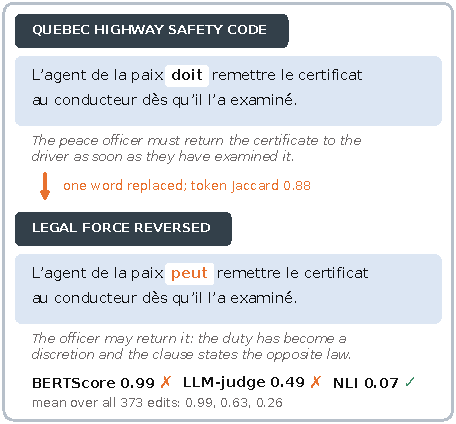
\includegraphics[width=\columnwidth]{figs/teaser.pdf}
\end{figure}

This article makes four contributions. First, it states a four-part validation
protocol for any scorer of legal meaning preservation, phrased over an arbitrary
scoring function rather than over an architecture. Second, it releases
\textsc{LexFlip}, a diagnostic set of \numedits\ minimally edited Quebec
statutory sentences whose legal force is reversed and whose surface form is
almost unchanged. Third, it administers the protocol to thirteen scorers,
including untrained similarity metrics, fine-tuned regressors and a prompted
large language model judge, and shows that correlation with human ratings and
sensitivity to a legally decisive edit come apart. Fourth, it reports what
happens when a metric is trained against the protocol, and finds that the
constraint is satisfied in distribution and not at all across a change of source
document.

\subsection{Related Work}\label{sec:related}

BLEU does not correlate with meaning preservation once sentence splitting is
involved \cite{sulem2018bleu}, and BERTScore \cite{zhang2019bertscore} and other
embedding metrics score high across \emph{all} alterations. \textsc{FrJudge}
\cite{beauchemin2025judgebert} is to our knowledge the only annotated resource
for legal meaning preservation in any language, and trained metrics fitted to
such corpora \cite{beauchemin2023meaningbert} are our point of departure.
Closest in method, Chen and Eger \cite{chen2023menli} show similarity metrics are
not robust to meaning-changing edits while metrics based on natural language
inference repair much of the gap, and Mujahid et al.\ \cite{mujahid2026stress}
run the complementary experiment on factual consistency in summarization. No
prior challenge set we know of targets legal force, which is the property a
simplification of a statute or an insurance clause has to preserve and the one a
lay reader cannot check. We follow Bean et al.\ \cite{bean2025construct} and
Pacchiardi et al.\ \cite{pacchiardi2024cleverhans} on construct validity, Deutsch
et al.\ \cite{deutsch2021statistical} and Graham and Baldwin
\cite{graham2014williams} on statistics, and Xu and Jurgens
\cite{xu2026disagreement} on rating distributions.

\section{What Would Validate a Legal Meaning Metric?}\label{sec:protocol}

The four requirements below are stated for an arbitrary scorer $m(o,s)$ over an
original clause $o$ and a candidate simplification $s$; none presupposes an
architecture.

\paragraph{R1: a measured ceiling}
A correlation with human judgment means nothing until one knows what correlation
a human achieves. Where a corpus carries $k \geq 3$ ratings per item this is
free: hold out one rater, correlate their ratings against the mean of the other
$k-1$, average over the held-out position. That answers \emph{is the metric as
good as an expert?}; the Spearman--Brown reliability of the $k$-rater mean
answers \emph{is it as good as the aggregate label allows?} A metric can sit
above the first and below the second without being superhuman, since predicting
an average is easier than being a rater.

\paragraph{R2: identical supervision}
Comparisons here place an unsupervised cosine similarity and a fine-tuned
regressor in one table, decimal-scale the former, and report RMSE for both.
Decimal scaling fixes the range but neither the location nor the shape of the
distribution, so a similarity occupying $[0.7,1.0]$ records a large RMSE however
well it ranks, and the column measures supervision rather than judgment.
We instead fit a monotone map from raw score to human scale on the training
split alone; isotonic regression cannot improve a ranking, and rank statistics
move by at most $\isoDeltaRho$.

\paragraph{R3: a trivial-feature control}
Simplifications are usually shorter and the dominant annotated error category is
omission, so a rubric deducting score once per identified error yields a label
partly predictable from how many words disappeared. We require a supervised
baseline over surface features alone, fitted under R2.

\paragraph{R4: dissociation}
On naturally occurring pairs surface form and legal force vary together, the
confound the endpoint checks inherit. Let $s'$ be a perturbation of $s$ with
token Jaccard $J(s,s') \approx 1$ and legal force $L(s') \neq L(s)$, and $u$ an
unrelated sentence of the same register. We report the \emph{margin fraction}
$(\overline{m(s,s)} - \overline{m(s,s')}) /
 (\overline{m(s,s)} - \overline{m(s,u)})$, the share of the metric's own
identical-to-unrelated range spent on a legally decisive edit, which charges it
against the range it actually has rather than a nominal $[0,1]$. A metric
treating the flipped sentence as it treats an unrelated one scores $1$; a pure
overlap function scores near $0$. This is not the rate at which $(s,s)$ outranks
$(s,s')$, the weaker quantity: a metric can rank every item correctly while
moving a thousandth of its range.

\section{Materials and Methods}\label{sec:methods}

\subsection{The \textsc{LexFlip} Diagnostic}\label{sec:lexflip}

Source sentences come from two Quebec statutes held out from every corpus used
here, the Automobile Insurance Act and the Highway Safety Code, and each takes
one minimal edit that changes legal force while leaving the sentence intact. The
inventory is organised by legal effect, not by linguistic category. Six families
make up \emph{tier 1}, where the edit unambiguously changes who is bound, what
is covered or how much: modality (\emph{doit} $\leftrightarrow$ \emph{peut}),
party (\emph{l'assur\'e} $\leftrightarrow$ \emph{l'assureur}), polarity
(dropping \emph{ne \dots pas}), quantum ($\times 10$), scope (\emph{tous les}
$\rightarrow$ \emph{certains}) and temporal (\emph{avant} $\leftrightarrow$
\emph{apr\`es}); \emph{tier 2} connective and class shifts are reported
separately. The diagnostic would fail if a metric could find the edited item by
noticing that it reads badly, so perturbations introducing a grammatical
artefact are filtered by a conservative French well-formedness check that flags
none of the $400$ unmodified sources. The result is \numedits\ pairs
(\numeditsTierOne\ tier 1) with mean token Jaccard \meanjaccard, none below
\minjaccard. Table~\ref{tab:examples} gives one sample per rule.

For each $s$ with perturbation $s'$ we score $(s,s)$, $(s,s')$ and $(s,u)$ for
an unrelated $u$ from the same statutes, min--max normalise per metric so the
two probes anchor the range, and take the margin from the three means.

\begin{table}
\centering
\caption{\textsc{LexFlip} samples, one per perturbation rule, with the edited
span in bold. Each remains fluent and statutory in register, shares almost all
of its tokens with the original, and states a different rule of
law.}\label{tab:examples}
\small
\setlength{\tabcolsep}{4pt}
\begin{tabular}{@{}p{0.97\columnwidth}@{}}
\toprule
\emph{peut} $\rightarrow$ \emph{doit} \hfill \emph{tier 1} \\[1pt]
\footnotesize $o$: La Société peut refuser une indemnité, en réduire le montant, en suspendre ou en cesser le paiement dans les cas suivants: 1. \\[1pt]
\footnotesize $s'$: La Société \textbf{doit} refuser une indemnité, en réduire le montant, en suspendre ou en cesser le paiement dans les cas suivants: 1. \\
\midrule
\emph{doit} $\rightarrow$ \emph{peut} \hfill \emph{tier 1} \\[1pt]
\footnotesize $o$: Le candidat doit toutefois réussir les examens de compétence visés à l'article 67 pour obtenir un permis de conduire pour motocyclette. \\[1pt]
\footnotesize $s'$: Le candidat \textbf{peut} toutefois réussir les examens de compétence visés à l'article 67 pour obtenir un permis de conduire pour motocyclette. \\
\midrule
drop \emph{ne \dots pas} \hfill \emph{tier 1} \\[1pt]
\footnotesize $o$: Les feux visés au paragraphe 2\textdegree{} ne sont pas requis pour tout véhicule dont la largeur excède 2,03 mètres. \\[1pt]
\footnotesize $s'$: Les feux visés au paragraphe 2\textdegree{} sont requis pour tout véhicule dont la largeur excède 2,03 mètres. \\
\midrule
\emph{avant} $\leftrightarrow$ \emph{apr\`es} \hfill \emph{tier 1} \\[1pt]
\footnotesize $o$: Elle n'est pas due avant le septième jour qui suit celui de l'accident, sauf dans le cas prévu au troisième alinéa de l'article 57. \\[1pt]
\footnotesize $s'$: Elle n'est pas due \textbf{après} le septième jour qui suit celui de l'accident, sauf dans le cas prévu au troisième alinéa de l'article 57. \\
\midrule
\emph{tous les} $\rightarrow$ \emph{certains} \hfill \emph{tier 1} \\[1pt]
\footnotesize $o$: Un agent de la paix peut enlever ou faire enlever aux frais du propriétaire toute chose utilisée en contravention au présent article. \\[1pt]
\footnotesize $s'$: Un agent de la paix peut enlever ou faire enlever aux frais du propriétaire \textbf{certaine} chose utilisée en contravention au présent article. \\
\bottomrule
\end{tabular}
\end{table}

\subsection{Scorers Evaluated}\label{sec:scorers}

Only French-capable metrics are administered, since scoring English-only ones on
French confounds coverage with quality. The set covers three families, named in
Table~\ref{tab:challenge}: BERTScore \cite{zhang2019bertscore} over CamemBERTv2
and FlauBERT, in F1 and recall-only variants since recall targets omission; four
sentence-embedding cosines (LaBSE, multilingual E5-base,
paraphrase-multilingual-mpnet and Sentence-CamemBERT); and bidirectional natural
language inference with mDeBERTa-XNLI \cite{laurer2024nli}, where failure of
$o \Rightarrow s$ signals hallucination and of $s \Rightarrow o$ omission, the
two dominant categories of the legal error taxonomy. We add token Jaccard and
the surface features of R3.

\subsection{The \textsc{FrJudge} Corpus and Its Reconstruction}\label{sec:corpus}

The diagnostic answers R4. We run the other three on \textsc{FrJudge}
\cite{beauchemin2025judgebert}, 297 insurance clauses simplified by
\texttt{gpt-4-turbo-2024-04-09} and rated by five law students on legal meaning
($1$--$10$), then ask whether the two kinds of evidence agree. The public
release drops annotator identity, making R1 impossible downstream, so we rebuild
the corpus from the raw Prodigy export, recovering the five annotators
(pseudonymised A--E) and reproducing the published pairwise agreement of
$25.96\%$. The same export carries the source document of each clause, which the
public release also drops and which Section~\ref{sec:grouped} uses to build a
document-grouped split.

Splits are $178/30/89$ pairs for training, development and test, drawn under ten
seeds for the unsupervised comparison and five for the trained models. Isotonic
calibration under R2 is fitted on the training split alone and never on the
split a number is reported from.

\subsection{A Prompted Judge}\label{sec:judgemethod}

A prompted model given the annotators' rubric \cite{enguehard2025lemaj} is the
natural competitor to a fine-tuned 112M-parameter encoder. We score each pair
with \texttt{deepseek-chat} under the \textsc{FrJudge} scale, a ten-point
judgment deducting one point per identified legal error, in its own request so
the judge never sees the probe condition, $K=5$ times, and average the samples.
Three prompt wordings are compared: the \textsc{FrJudge} rubric in French, the
same rubric in English over the same French text, and a bare instruction with
the four-type error taxonomy removed. A reasoning model
(\texttt{deepseek-reasoner}) is run under the identical rubric and items as a
capability control. The full protocol is $\judgeCalls$ calls costing
\$$\judgeCost$.

\subsection{Trained Metric Variants}\label{sec:variants}

The protocol so far audits scorers that already exist. It also has implications
for how one would fit a new one, and we test two of them. The first follows from
R1: the gold label is the mean of five ratings whose median spread is
\medianRange\ points, so fitting a scalar regressor to that mean asks the model
to predict a quantity none of the annotators asserted, and rewards predicting
the centre. The second follows from R4: if a diagnostic identifies a deficiency,
the obvious response is to train against it.

The seven configurations share an encoder (CamemBERTv2-base), splits, schedule
and seeds, and differ only in the target and the loss.

\begin{itemize}\itemsep2pt
\item \textbf{Scalar} (the conventional objective): mean squared error against
      the mean rating.
\item \textbf{Distributional}: a ten-way head trained with KL divergence against
      the empirical rating histogram, following Uma et al.\ \cite{uma2021learning}
      and Peterson et al.\ \cite{peterson2019human}. The reported score is the
      distribution's expectation, so it is directly comparable, but the model
      additionally exposes its spread.
\item \textbf{Annotator-aware}: five regression heads, one per annotator,
      averaged at inference. This lets the model represent the lenient and
      strict populations of Section~\ref{sec:ceiling} separately instead of
      averaging them away.
\item \textbf{Quantile}: a pinball loss \cite{koenker1978regression} at
      $\tau=0.25$. The asymmetry is deliberate. A metric that \emph{overshoots}
      the human rating is permissive of bad simplifications, while one that
      undershoots is merely strict, and in a legal setting those errors are not
      symmetric; a quantile objective encodes that preference in the loss rather
      than hoping it emerges.
\item \textbf{Multi-task}: the scalar head plus an auxiliary characterization
      head, trained against the majority vote of the five annotators, which
      spans 17 of the rubric's 18 classes (the eighteenth never carries a
      majority). The characterization labels are collected in \textsc{FrJudge}
      and then discarded; since the published rubric has annotators characterize
      a clause \emph{before} scoring it, the label plausibly carries information
      about the score.
\item \textbf{DA}: the scalar objective with the identical/unrelated
      augmentation in current use added to the training mixture, unchanged.
\item \textbf{DA+LexFlip}: \textbf{DA} plus minimally-edited negatives generated
      from \textsc{FrJudge} originals by the rules of Section~\ref{sec:lexflip},
      disjoint from the diagnostic's own sentences.
\end{itemize}

Correlation and RMSE are computed \emph{only} on the human-annotated test split,
never on a split containing augmentation. This matters: adding identical pairs
(label 10) and unrelated pairs (label 1) to the evaluation set inflates label
variance at the extremes, which raises Pearson $r$ for every metric without any
improvement in judgment. A table that does not separate the two shows the
signature clearly, in that a metric's $r$ and its RMSE improve and worsen
together rather than moving as one. Augmentation here affects training only, and
the three diagnostic regimes are reported separately as pass rates.

\subsection{Statistical Procedures}\label{sec:stats}

The test split holds $\testN$ items, at which size the smallest correlation
reliably distinguishable from $r=0.46$ at $80\%$ power is $\mindetect$. The
unsupervised metrics and the length feature correlate with the \emph{same} human
label on the \emph{same} $297$ items, and with each other, so a two-sample test
on Fisher-transformed correlations would be anticonservative; we use the
Williams test \cite{graham2014williams}, which corrects for that dependence.
Confidence intervals on correlations are bootstrap intervals over items.
Trained models are reported as means and standard deviations over five seeds and
unsupervised comparisons over ten, and we treat any difference smaller than that
spread as unresolved.

Every number we report is produced by a single pipeline that runs end to end on
a laptop; the largest model involved is CamemBERTv2-base (112M parameters) and
no GPU cluster is required. Training runs use Apple MPS kernels, which are not
bitwise deterministic, so a fixed seed reproduces a run only approximately:
repeat runs of the scalar configuration at seed $42$ differ in test-set $r$ by
several hundredths, comparable to the spread across seeds. Anyone reproducing
this on CUDA should expect tighter agreement and correspondingly narrower error
bars.

\subsection{Use of Generative AI}\label{sec:aidisclosure}

Generative AI enters this work in two distinct roles, and we separate them
because only one is a result. As an \emph{object of study},
\texttt{deepseek-chat} and \texttt{deepseek-reasoner} are scored as prompted
judges under the protocol of Section~\ref{sec:judgemethod}, and
\texttt{gpt-4-turbo-2024-04-09} produced the simplifications in \textsc{FrJudge}
before this work began. Separately, a large language model assistant was used to
rephrase passages of the manuscript for clarity. No AI system is an author. The
author designed the study, verified every reported number against the released
result files, and takes full responsibility for the content of this article,
including any part produced with the help of such a tool.

\begin{table*}
\centering
\caption{\textsc{LexFlip}, min--max normalised per metric. \emph{discrim.} is
the share of items ranked correctly (identical $>$ edited), \emph{margin} the
fraction of the identical-to-unrelated range spent on the legal
edit.}\label{tab:challenge}
\footnotesize
\setlength{\tabcolsep}{4pt}
\begin{tabular}{lrrrrr}
\toprule
Metric & identical & \textsc{LexFlip} & unrelated & discrim.\% & margin \\
\midrule
NLI-bidirectional (min) & 0.784 & 0.265 & 0.010 & 93.3 & 0.670 \\
NLI-bwd (no omission) & 0.784 & 0.432 & 0.042 & 77.2 & 0.473 \\
NLI-fwd (no hallucination) & 0.784 & 0.469 & 0.043 & 77.7 & 0.424 \\
LLM-judge (deepseek-chat, k=5) & 1.000 & 0.632 & 0.006 & 86.3 & 0.370 \\
surface: token Jaccard & 1.000 & 0.928 & 0.089 & 99.2 & 0.079 \\
LaBSE & 1.000 & 0.972 & 0.292 & 100.0 & 0.039 \\
BERTScore-FlauBERT & 1.000 & 0.979 & 0.393 & 100.0 & 0.035 \\
mE5-base & 1.000 & 0.975 & 0.266 & 100.0 & 0.034 \\
Para-mUSE-mpnet & 1.000 & 0.981 & 0.312 & 100.0 & 0.028 \\
Sentence-CamemBERT & 1.000 & 0.983 & 0.316 & 100.0 & 0.024 \\
BERTScore-CamemBERTv2-Recall & 1.000 & 0.983 & 0.240 & 100.0 & 0.023 \\
BERTScore-CamemBERTv2 & 1.000 & 0.982 & 0.193 & 100.0 & 0.022 \\
surface: $-|\,|s|-|o|\,|$ & 1.000 & 0.997 & 0.718 & 11.3 & 0.011 \\
\bottomrule
\end{tabular}
\end{table*}

\section{Results}\label{sec:results}

\subsection{Similarity Metrics Fail the Dissociation}\label{sec:diagnostic}

Every \emph{similarity}-based metric fails, and fails almost completely
(Table~\ref{tab:challenge}). The seven embedding and BERTScore variants spend
between $\simMarginLo$ and $\bertMargin$ of their working range on an edit that
reverses the law: BERTScore over CamemBERTv2 places a sentence saying the
opposite of the original at $0.982$, where the original sits at $1.000$ and an
unrelated statute at $0.193$. Token Jaccard, at $0.079$, is in the same regime,
which is the point: these are overlap functions, exactly as
Section~\ref{sec:protocol} says they must be. Their \emph{discrimination} rates
are uninformative for the same reason, the seven ranking the identical pair
first $100\%$ of the time by a margin that carries no decision. Bidirectional
NLI does not fail: it spends $\maxMargin$ of its range on the edit, ranks
correctly on $93.3\%$ of items, and places a flipped sentence nearer the
unrelated pair than the identical one. Figure~\ref{fig:challenge} shows the same
result as a picture: for every similarity metric the flipped sentence sits hard
against the identical pair, at the wrong end of the metric's own range.

\begin{figure}
\centering
\caption{\textsc{LexFlip}. For each metric the grey bar spans its score on an
unrelated pair (dark circle) to its score on an identical pair (blue circle):
its full working range. The red diamond is where it places a sentence whose
legal force has been reversed by a single word. A metric that measured legal
meaning would put the diamond at the left end. Every similarity-based metric
puts it at the right, hard against the identical pair. Only the four scorers
above the dashed rule, the three NLI variants and the prompted judge, move it
appreciably. Metric names are abbreviated; Table~\ref{tab:challenge} gives them
in full, with the margin column repeated at the right here.}\label{fig:challenge}
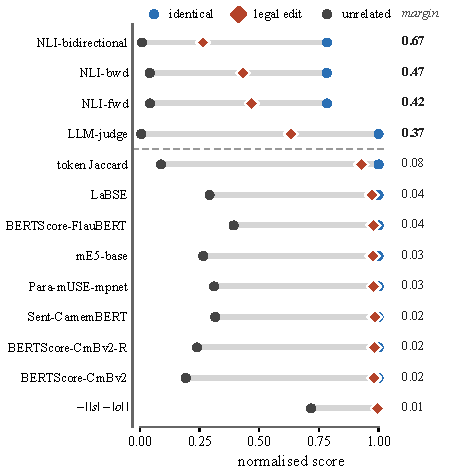
\includegraphics[width=\columnwidth]{figs/challenge.pdf}
\end{figure}

\paragraph{The existing checks would have excluded it}
Note where NLI's identical score sits: $0.784$, and not as a normalisation
artefact. In raw terms mDeBERTa assigns a mean entailment of $\nliIdentRaw$ to a
sentence paired with \emph{itself}, clearing the $99\%$ bar the identical-pair
convention requires on only $\nliIdentPass\%$ of items, against $100\%$ for
every BERTScore and embedding metric. The metric that best tracks legal meaning
is the one convention would \emph{disqualify}. Saturation on identical input is
easy to build, every overlap function having it by construction: report it, but
do not filter on it.

\subsection{Which Edits Are Detected}\label{sec:rules}

No perturbation rule is reliably detected (Table~\ref{tab:rules}). Averaged over
the \nMetricsChallenged\ scorers the best rule, dropping \emph{ne \dots pas},
reaches $\bestRuleMargin$, and the party swap between insurer and insured
reaches $\partyMarginAll$. Two details behind that party-swap figure are worth
stating. The two directions of the swap draw mean margins of $0.046$ and
$-0.005$ on $11$ and $3$ items respectively, which is why we pool them rather
than report either cell on its own: over all $\nParty$ party-swap items the
seven similarity metrics spend $\partyMargin$ of their range, with a per-metric
spread of $\partyMarginLo$--$\partyMarginHi$, against $\ruleMarginMeanSim$ for
those same seven metrics across all rules. The contrast is milder on this
restricted basis than the all-metric figures suggest, because the similarity
family has almost no range to spend on any rule.

We also tested whether the residual ordering across rules is explained by the
size of the edit in characters, and found no relationship ($r=\ruleSizeR$ over
the \nRules\ rules, $95\%$ CI $[\ruleSizeLo, \ruleSizeHi]$). With \nRules\ rules
of unequal frequency the ordering is not itself well determined, so we report it
descriptively; the robust observation is the ceiling on detectability, not the
ranking.

\begin{table}
\centering
\caption{\textsc{LexFlip} margin by perturbation rule, averaged over the metrics
in Table~\ref{tab:challenge}. \emph{worst} is the lowest margin any single
metric assigns that rule. A margin of $1$ would mean the metric treats a legally
flipped sentence exactly as it treats an unrelated one.}\label{tab:rules}
\small
\setlength{\tabcolsep}{4pt}
\begin{tabular}{lrrr}
\toprule
Perturbation & $n$ & mean margin & worst \\
\midrule
drop \emph{ne \dots pas} & 21 & 0.333 & 0.032 \\
\emph{avant} $\leftrightarrow$ \emph{apr\`es} & 9 & 0.272 & 0.006 \\
amount $\times$ 10 & 21 & 0.256 & 0.025 \\
\emph{doit} $\rightarrow$ \emph{peut} & 82 & 0.241 & 0.015 \\
\emph{sauf si} $\rightarrow$ \emph{si} & 10 & 0.225 & 0.014 \\
\emph{peut} $\rightarrow$ \emph{doit} & 111 & 0.167 & 0.018 \\
\emph{tous les} $\rightarrow$ \emph{certains} & 42 & 0.153 & 0.017 \\
\emph{et} $\rightarrow$ \emph{ou} & 27 & 0.069 & 0.007 \\
\emph{ou} $\rightarrow$ \emph{et} & 26 & 0.069 & 0.004 \\
\emph{assureur} $\rightarrow$ \emph{assur\'e} & 11 & 0.046 & 0.007 \\
\emph{automobile} $\leftrightarrow$ \emph{v\'ehicule} & 10 & 0.027 & -0.025 \\
\emph{assur\'e} $\rightarrow$ \emph{assureur} & 3 & -0.005 & -0.086 \\
\midrule
\textbf{All} & 373 & \textbf{0.155} & -- \\
\bottomrule
\end{tabular}
\end{table}

\subsection{Disagreement and the Human Ceiling}\label{sec:ceiling}

Krippendorff's $\alpha$ for legal meaning is $0.104$ under the \emph{nominal}
coefficient, the one conventionally reported here, and $\alphaOrd$ under the
\emph{ordinal} one appropriate to an ordered scale
\cite{krippendorff2004content}; Table~\ref{tab:agreement} gives all three
annotation dimensions, and our nominal figures reproduce the published ones. The
ordinal coefficient is computed with the same library and the same reliability
matrix as the nominal one, so the difference between $0.104$ and $\alphaOrd$ is
attributable to the distance function alone.

What remains after that correction is structural: the annotators separate into
two stable populations, B, C and D averaging $\lenientMean$ against
$\strictMean$ for A and E, and \pctSpreadSix\ of pairs span at least $6$ points
(Figure~\ref{fig:disagree}). Averaging leaves a target with standard deviation
$\labelSd$, the condition under which a regressor predicting the middle scores
well. Correlating each annotator against the mean of the other four gives a
ceiling of $\ceilR$ (RMSE $\ceilRmse$), with the held-out annotators ranging
from $0.524$ to $0.680$ (Table~\ref{tab:ceiling}); exceeding that ceiling is not
superhuman, the bound for predicting that mean being its own reliability,
$\sbRel$ by Spearman--Brown, so a metric can approach
$\sqrt{\sbRel}=\sbSqrt$.

\begin{table}
\centering
\caption{Krippendorff's $\alpha$ on \textsc{FrJudge}. Legal meaning is an
ordinal ten-point scale, for which the nominal coefficient is not the
appropriate measure. \emph{prev.}\ is the value reported by Beauchemin et al.\
\cite{beauchemin2025judgebert}.}\label{tab:agreement}
\small
\setlength{\tabcolsep}{4pt}
\begin{tabular}{lrrr}
\toprule
Dimension & \multicolumn{2}{c}{Krippendorff's $\alpha$} & Reported \\
\cmidrule(lr){2-3}
 & nominal & appropriate & prev. \\
\midrule
Simplicity level & 0.183 & 0.183 & 0.18 \\
Characterization & 0.552 & 0.552 & 0.55 \\
Legal meaning & 0.104 & \textbf{0.325} & 0.10 \\
\bottomrule
\end{tabular}
\end{table}

\begin{table}
\centering
\caption{Leave-one-annotator-out ceiling on \textsc{FrJudge} ($n=297$). A
single expert predicts the consensus of the other four at $r=\ceilR$, and the
best-agreeing pair of annotators reaches $r=\bestPairR$.}\label{tab:ceiling}
\small
\setlength{\tabcolsep}{4pt}
\begin{tabular}{lrrr}
\toprule
Held-out & $r$ (95\% CI) & $\rho$ & RMSE \\
\midrule
A & 0.524 [0.44, 0.60] & 0.551 & 3.93 \\
B & 0.569 [0.48, 0.65] & 0.586 & 3.05 \\
C & 0.680 [0.60, 0.75] & 0.725 & 2.75 \\
D & 0.601 [0.52, 0.67] & 0.557 & 3.08 \\
E & 0.612 [0.55, 0.67] & 0.679 & 3.56 \\
\midrule
\textbf{Mean (ceiling)} & \textbf{0.597} & 0.620 & 3.27 \\
Best pair (C-D) & 0.606 & -- & -- \\
Mean pairwise & 0.462 & -- & -- \\
\bottomrule
\end{tabular}
\end{table}

\begin{figure*}
\centering
\caption{Disagreement in \textsc{FrJudge}. (a) The five annotators form two
populations: B, C, D (blue) rate legal preservation about three points higher
than A and E (red) across the whole corpus. (b) Sorted within-item range; the
median item spans \medianRange\ points of a ten-point scale. (c) A single
annotator predicts the consensus of the other four at $r=\ceilR$ (bar; whiskers
give the range over the five held-out annotators), and the best-agreeing pair
reaches $r=\bestPairR$.}\label{fig:disagree}
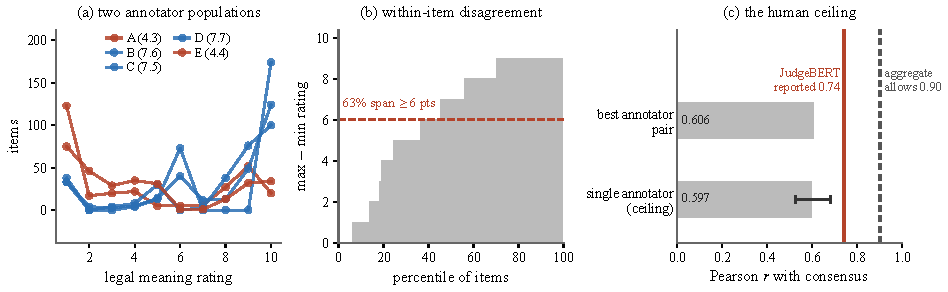
\includegraphics[width=\textwidth]{figs/disagreement.pdf}
\end{figure*}

\begin{table*}
\centering
\caption{Calibrated comparison on the \textsc{FrJudge} test split ($\testN$
items), mean over 10 seeds. RMSE$_{\text{raw}}$ is the decimal-scaling protocol
in current use; RMSE$_{\text{cal}}$ fits an isotonic map on the training split.
$r$ and $\rho$ are both computed after calibration; being monotone, the map
leaves $\rho$ almost unchanged (at most $\isoDeltaRho$) but shifts $r$ by up to
$\isoDeltaR$.}\label{tab:baselines}
\small
\setlength{\tabcolsep}{4pt}
\begin{tabular}{lrrrrr}
\toprule
Metric & $r$ & $\rho$ & RMSE$_{\text{raw}}$ & RMSE$_{\text{cal}}$ & over\% \\
\midrule
\multicolumn{6}{l}{\emph{Unsupervised, French-capable}}\\
BERTScore-CamemBERTv2 & 0.291$_{\pm0.09}$ & 0.326 & 2.62 & 2.36 & 49.3 \\
BERTScore-CamemBERTv2-Recall & 0.352$_{\pm0.12}$ & 0.398 & 2.59 & 2.30 & 47.2 \\
BERTScore-FlauBERT & 0.482$_{\pm0.08}$ & 0.459 & 2.16 & 2.12 & 49.4 \\
LaBSE & 0.409$_{\pm0.06}$ & 0.402 & 2.33 & 2.21 & 47.2 \\
Sentence-CamemBERT & 0.296$_{\pm0.05}$ & 0.287 & 2.68 & 2.31 & 49.3 \\
Para-mUSE-mpnet & 0.252$_{\pm0.08}$ & 0.266 & 2.88 & 2.35 & 47.2 \\
mE5-base & 0.358$_{\pm0.08}$ & 0.356 & 2.52 & 2.26 & 48.0 \\
NLI-fwd (no hallucination) & 0.368$_{\pm0.06}$ & 0.352 & 3.85 & 2.25 & 49.3 \\
NLI-bwd (no omission) & 0.340$_{\pm0.09}$ & 0.355 & 3.70 & 2.28 & 46.9 \\
NLI-bidirectional (min) & 0.395$_{\pm0.07}$ & 0.405 & 3.74 & 2.22 & 46.6 \\
\midrule
\multicolumn{6}{l}{\emph{Trivial surface features}}\\
$-|\,|s|-|o|\,|$ (length difference) & 0.641$_{\pm0.04}$ & 0.624 & 3.25 & 1.85 & 47.0 \\
Token Jaccard & 0.303$_{\pm0.06}$ & 0.331 & 3.34 & 2.34 & 48.0 \\
Length ratio & 0.580$_{\pm0.05}$ & 0.560 & 3.43 & 1.97 & 49.1 \\
Surface-Ridge (10 features, supervised) & 0.621$_{\pm0.05}$ & 0.588 & 1.89 & 1.89 & 45.8 \\
\midrule
\multicolumn{6}{l}{\emph{Prompted LLM judge}}\\
LLM-judge (deepseek-chat, k=5) & 0.755$_{\pm0.05}$ & 0.753 & 2.93 & 1.57 & 43.9 \\
\midrule
\textbf{Human ceiling} (one annotator) & \textbf{0.597} & 0.620 & -- & 3.27 & -- \\
\bottomrule
\end{tabular}
\end{table*}

\subsection{Identical Supervision, and a Trivial Control}\label{sec:baselines}

Calibration collapses most of the RMSE gap uncalibrated comparisons record
(Table~\ref{tab:baselines}): the metrics were not as far from human judgment as
such tables suggest, merely on a different scale. And a ridge over word counts
and token overlap reaches $r=\surfR$, at the human ceiling and above every
semantic metric we test, the best reaching $r=0.482$. Only two scorers beat it,
and neither is semantic: the prompted judge below, and the bare length
difference at $r=0.641$. Under the Williams test every one of the ten
unsupervised neural metrics is significantly \emph{worse} than that length
feature (Table~\ref{tab:significance}: $t$ between $2.61$ and $6.33$,
$p \leq 0.010$), so the ordering is not an artefact of sampling. This says less about the corpus than about what the
\emph{annotation} rewards, score being reduced once per identified error and the
most frequent error type, omission, correlating strongly with becoming shorter.

\begin{table}
\centering
\caption{Williams tests against the trivial length baseline
$\ell = -|\,|s|-|o|\,|$, which reaches $r=0.613$ with the human label $h$ over
all $297$ items. $r(m,\ell)$ is each metric's correlation with the length
feature itself, the dependence the test corrects for. Positive $t$ favours
$\ell$.}\label{tab:significance}
\footnotesize
\resizebox{\columnwidth}{!}{\setlength{\tabcolsep}{4pt}
\begin{tabular}{lrrrr}
\toprule
Neural metric $m$ & $r(m,h)$ & $r(m,\ell)$ & $t$ & $p$ \\
\midrule
BERTScore-CamemBERTv2 & 0.344 & 0.349 & 5.05 & $<$0.001 \\
BERTScore-CamemBERTv2-Recall & 0.396 & 0.443 & 4.43 & $<$0.001 \\
BERTScore-FlauBERT & 0.484 & 0.389 & 2.61 & 0.010 \\
LaBSE & 0.424 & 0.362 & 3.66 & $<$0.001 \\
Sentence-CamemBERT & 0.222 & 0.148 & 6.33 & $<$0.001 \\
Para-mUSE-mpnet & 0.225 & 0.159 & 6.32 & $<$0.001 \\
mE5-base & 0.318 & 0.316 & 5.40 & $<$0.001 \\
NLI-fwd (no hallucination) & 0.320 & 0.388 & 5.66 & $<$0.001 \\
NLI-bwd (no omission) & 0.307 & 0.258 & 5.36 & $<$0.001 \\
NLI-bidirectional (min) & 0.365 & 0.350 & 4.68 & $<$0.001 \\
\bottomrule
\end{tabular}}
\end{table}

\subsection{The Prompted Judge}\label{sec:judge}

Under R2 the prompted judge reaches $r=\judgeR_{\pm\judgeRsd}$, above the length
feature and our ceiling (a redraw gave $\repRcalTwo$). On \textsc{LexFlip} it
scores the identical pair at $\judgeIdent$ and the unrelated pair at
$\judgeUnrel$, flawless on the two checks jointly satisfiable by overlap, then
awards a clause whose legal force has been reversed $\judgeEdit$ out of ten, a
margin of $\judgeMargin$.

The rubric, not the model, limits this. With the model fixed the margin moves
from $\promptMarginLo$ under the rubric-faithful prompt to $\promptMarginHi$
under a bare instruction stripping the four-type taxonomy, against $0.002$ for a
redraw, and the correlation moves the other way, from $\promptRubricR$ to
$\promptBareR$. Score is reduced \emph{once per identified error}, so a clause
reversal is one incoherence and the penalty is capped near the top of the scale.
Substituting a reasoning model under the identical rubric and items does not
help: \texttt{deepseek-reasoner} gives $r=\reasonerR$ against $\chatKoneR$ and
margin $\reasonerMargin$ against $\chatKoneMargin$ at matched sampling, so the
shortfall is not a matter of the model thinking harder.

One behaviour survives every configuration: \emph{peut} for \emph{doit} scores
$\asymWeaken$ while the reverse scores $\asymStrengthen$, though both change the
law by the same construction. The gap ranges from $\asymGapLo$ to $\asymGapHi$
across the \nConfigs\ configurations we ran. The judge therefore tracks legal
\emph{severity} rather than legal \emph{equivalence}, penalising a clause that
becomes more permissive and forgiving one that becomes more demanding.

\paragraph{The judge as a sixth annotator}
Because the judge emits on the annotators' scale it can be placed inside the
panel rather than only beside the metrics. Its mean rating is
$\judgeMeanRating$, against a human panel spanning $\strictMean$ to
$\lenientMean$, so it is more lenient than any human and far less dispersed. Yet
its mean correlation with the five annotators is $\judgeHumanR$, higher than the
mean human-to-human correlation of $\humanHumanR$. Adding it as a sixth coder
nonetheless \emph{lowers} ordinal $\alpha$ from $\alphaOrd$ to
$\judgeAlphaPanel$: it tracks the consensus without belonging to the
distribution. Against its own five samples it is far more self-consistent than
the humans are with each other ($\alpha=\judgeAlphaSelf$ versus $\alphaOrd$),
and averaging the samples is not cosmetic, since correlation against the human
mean climbs from $\judgeKone$ at $K=1$ to $\judgeKfive$ at $K=5$. Its
rubric-level explanations show the same pattern: on identical pairs it reports
an error in $\judgeErrIdent\%$ of samples, and on \textsc{LexFlip} it reports
some error in $\judgeErrEdit\%$ and names \emph{incoh\'erence}, the correct type
for a meaning-reversing edit, in $\judgeErrIncoh\%$. Of six rules for merging
the judge with bidirectional NLI, every calibration fitted on the training split
alone and the diagnostic never entering the fit, none beats both parents on both
axes; the best, a weighted blend at $w=\hybridW$, reaches $r=\hybridR$ and
margin $\hybridMargin$, gains smaller than the redraw-to-redraw variation. We
report this as a negative result rather than proposing a metric.

\begin{table*}
\centering
\caption{Trained metrics, mean over 5 seeds, evaluated on the human-annotated
test split only. \emph{ident.}\ and \emph{unrel.}\ are the two sanity checks in
current use; \textsc{LexFlip} false-acceptance is the share of legally flipped
pairs still scored $\geq 7$ (``accurate'' under the published rubric). The
margin is the quantity defined in Section~\ref{sec:protocol}. It is shown as
`--' where a model places the identical and unrelated probes within one point of
each other, because a model with no working range has none to spend on the
edit.}\label{tab:models}
\small
\setlength{\tabcolsep}{4pt}
\begin{tabular}{lrrrrrrrr}
\toprule
Model & $r$ & $\rho$ & RMSE & over\% & ident.\ & unrel.\ & \multicolumn{2}{c}{\textsc{LexFlip}} \\
\cmidrule(lr){8-9}
 &  &  &  &  & pass & pass & false-acc.\ & margin \\
\midrule
JudgeBERT-Scalar (baseline) & 0.542$_{\pm0.08}$ & 0.280 & 2.48 & 25.4 & 0 & 0 & 0 & -- \\
JudgeBERT-Dist (soft labels) & 0.572$_{\pm0.03}$ & 0.578 & 1.99 & 42.9 & 0 & 0 & 69 & 0.015 \\
JudgeBERT-Annot (5 heads) & 0.534$_{\pm0.05}$ & 0.585 & 3.47 & 12.6 & 0 & 0 & 0 & -- \\
JudgeBERT-Quantile (tau=.25) & 0.553$_{\pm0.06}$ & 0.377 & 3.28 & 9.9 & 0 & 0 & 0 & -- \\
JudgeBERT-MT (+charact.) & 0.519$_{\pm0.06}$ & 0.232 & 2.51 & 26.3 & 0 & 0 & 0 & -- \\
\midrule
JudgeBERT-DA & 0.192$_{\pm0.25}$ & 0.112 & 2.31 & 42.5 & 0 & 77 & 18 & 0.019 \\
JudgeBERT-DA+LexFlip & 0.122$_{\pm0.10}$ & 0.174 & 2.60 & 35.3 & 0 & 69 & 0 & 0.051 \\
\midrule
\emph{NLI-bidirectional} (untrained) & 0.395 & 0.405 & 2.22 & 46.6 & 1 & -- & -- & \emph{0.670} \\
\textbf{Human ceiling} & \textbf{0.597} & 0.620 & 3.27 & -- & -- & -- & -- & -- \\
\bottomrule
\end{tabular}
\end{table*}

\subsection{What Training Against the Protocol Buys}\label{sec:training}

Table~\ref{tab:models} reports the grid of Section~\ref{sec:variants}, and the
first result is a negative one: no training target moves the correlation by more
than the scalar baseline's own spread across seeds ($\pm0.082$), which is itself
far smaller than the difference of roughly a quarter of a correlation point that
an $\testN$-item split can resolve. The differences that survive are in the
other columns. The distributional head is markedly steadier than the scalar head
it replaces ($\pm0.029$ against $\pm0.082$ over the same five seeds), reaches the
best RMSE in the table ($1.99$), and roughly doubles the rank correlation
($\rho=0.578$ against $0.280$), which is what one expects from a target carrying
the shape of the rating distribution and not only its mean. The quantile head
does precisely what it was asked to do: it overshoots the human label on $9.9\%$
of test items against $25.4\%$ for the scalar head, the lowest rate of any model
here. The risk asymmetry a legal setting calls for can therefore be written into
the loss rather than hoped for, and it costs nothing in correlation.

\paragraph{Trained constraints do not cross a change of document}
Every model in Table~\ref{tab:models} scores $0\%$ on the identical-pair check,
the two augmented ones included, although identical pairs are in their training
mixture; the augmented models pass the unrelated check on $77\%$ and $69\%$ of
probes and the un-augmented models on none. The asymmetry is the one our probe
design predicts. Our unrelated probes are drawn from the same two statutes the
training mixture draws its unrelated pairs from, so passing that check is an
in-distribution result; our identical probes are statutory sentences while the
mixture's identical pairs are \textsc{FrJudge} clauses, so passing that one
would require generalising across source documents, and no model does. The same
holds for the diagnostic: \textsc{DA+LexFlip}, trained on minimally-edited
negatives, reaches a margin of $0.051$ against $\maxMargin$ for untrained
bidirectional NLI, its negatives generated from \textsc{FrJudge} originals and
its probes from statutes. Training on a constraint buys satisfaction of it in
distribution and nothing at all across a change of source. The same separation
explains the augmented mixtures' correlations, which are the clearest effect in
the table: \textsc{DA} loses $0.350$ against the un-augmented baseline and
\textsc{DA+LexFlip} $0.420$, on five seeds out of five in both cases, and
\textsc{DA} varies by $\pm0.254$ across seeds, reaching $r=-0.188$ on one of
them.

One column should be read with care. \textsc{LexFlip} false-acceptance is the
share of flipped pairs still scored $\geq 7$, so it is confounded with where a
model puts its predictions overall. The distributional head's $69\%$ reflects a
head that scores high in general (its identical probes average $7.22$), and the
$0\%$ of the scalar heads reflects models that score low on everything, not
models that reject the edit.

\subsection{What Survives a Change of Document}\label{sec:grouped}

A metric meta-evaluation that never changes source document cannot distinguish
legal sensitivity from familiarity with a form. Random splitting lets clauses
from the same insurance form appear in both training and test, and insurance
forms are highly templated, so we rerun the scalar baseline and the two
augmented mixtures on a document-grouped split in which no source document
straddles the boundary, size-matched to the random split pair for pair. The
remaining four configurations differ from the baseline in what they are trained
to predict rather than in what they can exploit about a source form, so the
leakage they are exposed to is the same.

The comparison does not resolve. The scalar baseline's correlation falls from
$0.542$ on the random split to $0.454$ on the grouped one, a drop of $0.088$
that is in the direction leakage would predict, and it does not survive
inspection: the per-seed differences are $+0.169$, $-0.097$, $-0.416$, $-0.182$
and $+0.086$, so two of the five seeds \emph{improve} under the harder split and
the grouped spread ($\pm0.143$) is wider than the gap itself. The two augmented
mixtures move by $-0.002$ and $+0.026$, which is to say not at all. As a
control, the untrained NLI reference is fitted to nothing and should be
indifferent to how the corpus is partitioned; it moves from $0.395$ to $0.391$,
confirming that the two splits are otherwise comparable and that the variance
above is the models' and not the split's.

We therefore do not claim that document-level leakage inflates these
correlations, and we hold our own evidence to the standard
Section~\ref{sec:limits} applies elsewhere. What we can say is narrower and, we
think, more useful to anyone planning a successor corpus: \textsc{FrJudge} is
too small and too concentrated to answer the question. Its 297 pairs come from
only 21 source forms and the three largest hold $71\%$ of them, so the largest
form alone is $37\%$ of the corpus, larger than the $30\%$ test quota, and
always falls in training. The grouped test split is therefore always drawn from
the $188$ pairs that form leaves behind, at which size the seed-to-seed
variation swamps the effect being measured. A corpus intended to support an
out-of-domain claim needs its documents spread far more evenly, and this is the
aspect of the design we would change first.

\subsection{Stratifying by Length Change}\label{sec:buckets}

If a metric's correlation is concentrated in the items where the simplification
is much shorter, it is detecting deletion rather than legal change.
Table~\ref{tab:buckets} reports Pearson $r$ inside each tercile of
$|\,|s|-|o|\,|$. Within a tercile the length signal is largely held constant, so
a metric that retains its correlation there is using something other than
deletion; one whose correlation collapses was reading length all along. This is
a weaker form of the same dissociation logic as Section~\ref{sec:lexflip}: it
holds a confound approximately fixed by conditioning rather than exactly fixed
by construction.

\begin{table}
\centering
\caption{Correlation with the human label \emph{within} terciles of the absolute
length change, pooling test predictions over seeds. Restricting to a tercile
removes most of the length variance; a metric that measures legal meaning should
degrade far less than one that measures deletion.}\label{tab:buckets}
\small
\setlength{\tabcolsep}{4pt}
\begin{tabular}{lrrrr}
\toprule
& \multicolumn{3}{c}{$r$ within tercile} & \\
\cmidrule(lr){2-4}
Metric & small & medium & large & all \\
\midrule
$-|\,|s|-|o|\,|$ & 0.243 & 0.165 & 0.585 & 0.613 \\
BERTScore-FlauBERT & 0.198 & 0.449 & 0.413 & 0.484 \\
LaBSE & 0.174 & 0.532 & 0.240 & 0.424 \\
NLI-bidirectional & 0.058 & 0.269 & 0.291 & 0.365 \\
Surface-Ridge & 0.118 & 0.305 & 0.540 & 0.620 \\
JudgeBERT-Scalar & 0.042 & 0.149 & 0.602 & 0.496 \\
\bottomrule
\end{tabular}
\end{table}

The result qualifies Section~\ref{sec:baselines} in a way that cuts against our
own argument, and is worth stating carefully. The length feature's correlation
is overwhelmingly a \emph{between}-tercile effect: pooled over the corpus it
reaches $0.613$, but inside the small and medium terciles it falls to $0.243$
and $0.165$. Once items of comparable length change are compared with each
other, knowing the length change tells you little. It recovers to $0.585$ only
in the tercile where the simplification is much shorter than the original, which
is exactly where deletion is available to be detected. The neural baselines have
the opposite profile: in the medium tercile, where the length feature retains
almost nothing, BERTScore over FlauBERT holds $0.449$ against a pooled $0.484$
and LaBSE rises to $0.532$ against a pooled $0.424$. The supervised surface ridge
tracks the raw length feature bucket for bucket, which is what one would expect
if it is largely a length model with extra terms. The small tercile is hard for
everything, which we read as a floor effect rather than as a result: when the two
sentences are close to the same length, none of these signals has much to go on.

The honest reading is therefore narrower than ``legal meaning preservation is
length preservation''. The corpus-level ranking is dominated by length, and any
comparison that omits a length control will attribute to a metric what it should
attribute to that confound. But the neural metrics are not \emph{only} reading
length. Where the length signal is weakest, they are the ones that hold up.
Whatever they are reading in that stratum, it is not the length change. What
Section~\ref{sec:diagnostic} adds is that the residual signal they retain is
still not legal sensitivity, since the same metrics move almost not at all when
the law is changed and the length is held exactly fixed. The two analyses answer
different questions, and a metric has to survive both.

\begin{figure}
\centering
\caption{The two orderings come apart. Horizontally, calibrated correlation with
the human label, the quantity a conventional comparison selects on; vertically,
the share of working range spent on an edit that reverses the
law.}\label{fig:dissociation}
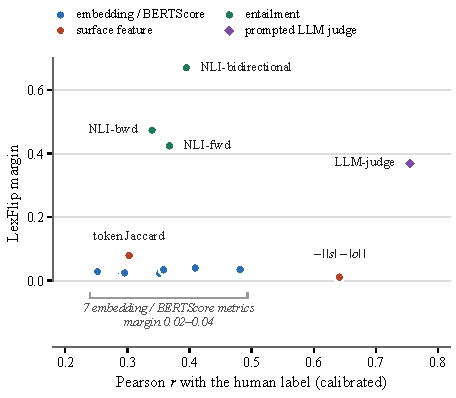
\includegraphics[width=0.82\columnwidth]{figs/dissociation.pdf}
\end{figure}

\subsection{Correlation and Legal Sensitivity Come Apart}\label{sec:dissociation}

Over the \nDissocAll\ scorers carrying both a calibrated $r$ and a margin the
rank correlation between them is $\rho=\dissocRhoAll$ ($95\%$ interval
$[\dissocRhoAllLo, \dissocRhoAllHi]$), an absence of resolution rather than a
demonstrated null; the extremes are the durable part. The length feature
outscores every semantic metric and has the lowest margin of anything we test
($\minMargin$), while bidirectional NLI sits mid-table on correlation and alone
reacts to the edit. The empty upper-right quadrant of
Figure~\ref{fig:dissociation} is the finding: nothing we test is both a good
predictor of the human label and sensitive to a legally decisive edit.

\section{Discussion}\label{sec:discussion}

A metric claiming to measure legal meaning should report three checks, not two:
identical pairs (saturation), unrelated pairs (bottoming out), and
\textsc{LexFlip} (does it move when, and only when, the law moves?). The first
two are jointly satisfiable by lexical overlap; the third is not, so a low
margin is a fixable deficiency rather than a limit of automatic evaluation. Only
legal sensitivity resists calibration: rank on it, and build the next metric on
a repaired entailment objective.

The practical consequences fall into three places. For anyone \emph{building} a
metric, the diagnostic says that the objective and not the encoder is what needs
changing. Seven configurations sharing an encoder and differing only in target
and loss move the correlation by less than seed noise, while an untrained
bidirectional entailment score, which is the only scorer here whose training
objective is about directional meaning containment rather than similarity,
outperforms all of them on the one axis that matters. For anyone
\emph{reporting} a metric, R2 and R3 are cheap and change conclusions: isotonic
calibration erases most of the RMSE gap that uncalibrated tables attribute to
supervision, and a length control moves a semantic metric from ``competitive
with humans'' to ``below a feature that counts words''. For anyone
\emph{deploying} a metric, the asymmetry the prompted judge shows is the sharpest
warning in the paper. It penalises a clause that becomes more permissive far more
than one that becomes more demanding, which is a defensible policy and a
disastrous default if it is not the policy anyone chose.

Two findings generalise beyond legal text. The first is that a validation
protocol built only from endpoint checks can be satisfied by construction, and
the repair, holding one variable fixed while moving the other, applies to any
evaluation where the property of interest is correlated with surface form in
naturally occurring data. The second is that training against a diagnostic buys
satisfaction of it in distribution and nothing across a change of source
document, which is a reason to keep such diagnostics out of training mixtures
and to treat them, as we do, as necessary conditions rather than benchmarks to
optimise. Both point at the same practical recommendation for whoever builds the
next corpus in this area. Source documents should be spread evenly enough that a
grouped split is possible, annotator identity should survive into the public
release so that a ceiling can be measured downstream, and a held-out set of
minimally edited negatives should be published alongside the ratings and kept
out of every training mixture, so that legal sensitivity can be reported next to
correlation rather than inferred from it.

\section{Limitations}\label{sec:limits}

Our \textsc{LexFlip} labels are definitional rather than annotated: we assert
that replacing \emph{doit} with \emph{peut} changes legal meaning rather than
having lawyers rate each perturbation. That is defensible for tier-1 edits,
reported separately from tier 2, but a small expert study would be stronger. The
edits are single and template-generated, so a system could be tuned to them
without acquiring general legal sensitivity, which is why the diagnostic is a
necessary condition and not a benchmark to optimise.

The same caveat bears on our best result. Our perturbations are largely
negation, modality, quantifier and antonym contrasts, close to what NLI training
data is built around, so bidirectional NLI's margin of $\maxMargin$ may reflect
familiarity with their \emph{form} rather than sensitivity to their legal
consequence. Yang et al.\ \cite{yang2026compared} give the general version: a
counterfactual edit isolates the variable of interest only against a
meaning-preserving paraphrase control, which we do not run and the next version
of the diagnostic should carry.

Finally, the diagnostic and the corpus comparison run on different text,
insurance forms against two statutes, and answer different questions; the judge
results rest on one model under a rubric reconstructed from the published
description, a load-bearing assumption given that wording alone moves the margin
by $\promptMarginRange$; and the ceiling is computed on all 297 items while model
correlations run on $\testN$-item splits, so ``model $>$ ceiling'' carries the
sampling uncertainty of both. The corpus itself is one language and one legal
system, and whether the same dissociation holds for common-law English drafting
is an open question our design cannot answer.

\section{Conclusion}\label{sec:conclusion}

Legal meaning preservation metrics are validated today by two checks that
lexical overlap satisfies by construction. We proposed a third that it cannot,
released \textsc{LexFlip} to administer it, and found that every similarity-based
metric in current use spends between $\simMarginLo$ and $\bertMargin$ of its own
working range on an edit that reverses a statutory obligation. Bidirectional NLI
is the exception at $\maxMargin$, and it is the family the identical-pair
convention would have excluded. On the only annotated corpus for this task a
supervised ridge over word counts matches a measured human ceiling and beats
every semantic metric, and a prompted judge exceeds the ceiling while awarding a
reversed clause $\judgeEdit$ out of ten. Correlation with human ratings and
sensitivity to a change in the law are, on the evidence here, close to
independent. Reporting both is the smallest change that would make the
difference visible, and repairing the entailment objective is where we would
look for the next metric.

\section*{Acknowledgement}\label{acknowledgement}

An earlier version of this work has been made available as a preprint on arXiv
\cite{baral2026lexflip}. The author thanks the authors of \textsc{FrJudge} for
releasing the corpus and the raw annotation export on which the reconstruction
in Section~\ref{sec:corpus} depends.

\section*{Funding Support}\label{funding-support}

This research received no specific grant from any funding agency in the public,
commercial, or not-for-profit sectors.

\section*{Ethical Statement}\label{ethical-statement}

This study does not contain any studies with human or animal subjects performed
by the author. It reuses an existing annotated corpus, \textsc{FrJudge}, whose
five annotators are pseudonymised as A--E throughout; our released code
pseudonymises annotator identifiers on load, and we ship the pseudonymisation
script for anyone redistributing a reconstruction.

Beauchemin et al.\ \cite{beauchemin2025judgebert} caution that their metric
informs a practitioner about legal meaning preservation rather than supplying a
complete juridical analysis, and our results sharpen that into a rule. A metric
that cannot distinguish \emph{doit} from \emph{peut} must not gate whether a
simplified clause is safe to publish, and the appropriate deployment is triage,
the ranking of clauses for human review, rather than certification. Nothing in
this article constitutes legal advice. The perturbed sentences we release are
deliberate misstatements of Quebec law, labelled as such in the distribution,
and are not statements of the law.

\section*{Conflicts of Interest}\label{conflicts-of-interest}

The author declares that he has no conflicts of interest to this work.

\section*{Data Availability Statement}\label{data-availability-statement}

The data and code that support the findings of this study are openly available
at \url{https://github.com/Nyvora-Vision-Labs/LEXFLIP}. The repository contains
the \textsc{LexFlip} generator and the released item set, the scoring harness,
the reconstruction of \textsc{FrJudge} from its raw export (which recovers
annotator identity and source document, both dropped from the public JSONL), the
document-grouped splits, and the result files behind every table in this
article. \textsc{FrJudge} itself is distributed by Beauchemin et al.\
\cite{beauchemin2025judgebert} and is not redistributed here.

%% The reference list is set flush to the foot of the page: \flushbottom undoes
%% the document-wide \raggedbottom for this last page, and the infinitely
%% stretchable gap between entries lets both columns run to the bottom margin.
\flushbottom
\begingroup
\setlength{\parskip}{0pt}
\AtBeginEnvironment{thebibliography}{\setlength{\itemsep}{0pt plus 1fill}}
%% Reference list for the JCLLT submission, kept in its own file the way
%% bib_main.tex and bib_supp.tex are, and typeset directly rather than
%% through BibTeX. Entries are in APA form, as the journal requires, and
%% stay in order of first citation so the first work cited is [1].
%% paper/citations.md is the authority for what each entry says.

\begin{thebibliography}{99}

\bibitem{magesh2025hallucinationfree} %
Magesh, V., Surani, F., Dahl, M., Suzgun, M., Manning, C. D., \& Ho, D. E.
(2025). Hallucination-free? Assessing the reliability of leading AI legal
research tools. \textit{Journal of Empirical Legal Studies}, \textit{22}(2),
216--242.

\bibitem{beauchemin2023meaningbert} %
Beauchemin, D., Saggion, H., \& Khoury, R. (2023). MeaningBERT: Assessing
meaning preservation between sentences. \textit{Frontiers in Artificial
Intelligence}, \textit{6}, 1223924.

\bibitem{beauchemin2025judgebert} %
Beauchemin, D., Albert-Rochette, M., Khoury, R., \& D\'eziel, P.-L. (2025).
JUDGEBERT: Assessing legal meaning preservation between sentences. In
\textit{Proceedings of the 2025 Conference on Empirical Methods in Natural
Language Processing} (pp.~92--118).

\bibitem{sulem2018bleu} %
Sulem, E., Abend, O., \& Rappoport, A. (2018). BLEU is not suitable for the
evaluation of text simplification. In \textit{Proceedings of the 2018 Conference
on Empirical Methods in Natural Language Processing} (pp.~738--744).

\bibitem{zhang2019bertscore} %
Zhang, T., Kishore, V., Wu, F., Weinberger, K. Q., \& Artzi, Y. (2019).
BERTScore: Evaluating text generation with BERT. \textit{arXiv preprint
arXiv:1904.09675}.

\bibitem{chen2023menli} %
Chen, Y., \& Eger, S. (2023). MENLI: Robust evaluation metrics from natural
language inference. \textit{Transactions of the Association for Computational
Linguistics}, \textit{11}, 804--825.

\bibitem{mujahid2026stress} %
Mujahid, Z. M., Wright, D., \& Augenstein, I. (2026). Stress testing factual
consistency metrics for long-document summarization. In \textit{Proceedings of
the 64th Annual Meeting of the Association for Computational Linguistics (Volume
1: Long Papers)} (pp.~31914--31933).

\bibitem{bean2025construct} %
Bean, A. M., Kearns, R. O., Romanou, A., Hafner, F. S., Mayne, H., Batzner, J.,
Foroutan Eghlidi, N., et al. (2026). Measuring what matters: Construct validity
in large language model benchmarks. \textit{Advances in Neural Information
Processing Systems}, \textit{38}.

\bibitem{pacchiardi2024cleverhans} %
Pacchiardi, L., Tesic, M., Cheke, L. G., \& Hern\'andez-Orallo, J. (2024).
Leaving the barn door open for Clever Hans: Simple features predict LLM
benchmark answers. \textit{arXiv preprint arXiv:2410.11672}.

\bibitem{deutsch2021statistical} %
Deutsch, D., Dror, R., \& Roth, D. (2021). A statistical analysis of
summarization evaluation metrics using resampling methods.
\textit{Transactions of the Association for Computational Linguistics},
\textit{9}, 1132--1146.

\bibitem{graham2014williams} %
Graham, Y., \& Baldwin, T. (2014). Testing for significance of increased
correlation with human judgment. In \textit{Proceedings of the 2014 Conference
on Empirical Methods in Natural Language Processing (EMNLP)} (pp.~172--176).

\bibitem{xu2026disagreement} %
Xu, Y., \& Jurgens, D. (2026). Beyond consensus: Perspectivist modeling and
evaluation of annotator disagreement in NLP. \textit{arXiv preprint
arXiv:2601.09065}.

\bibitem{laurer2024nli} %
Laurer, M., van Atteveldt, W., Casas, A., \& Welbers, K. (2024). Less
annotating, more classifying: Addressing the data scarcity issue of supervised
machine learning with deep transfer learning and BERT-NLI. \textit{Political
Analysis}, \textit{32}(1), 84--100.

\bibitem{krippendorff2004content} %
Krippendorff, K. (1996). \textit{Content analysis: An introduction to its
methodology}. TPB.

\bibitem{enguehard2025lemaj} %
Enguehard, J., Van Ermengem, M., Atkinson, K., Cha, S., Ghosh Chowdhury, A.,
Kallur Ramaswamy, P., Roghair, J., et al. (2025). LeMAJ (Legal LLM-as-a-Judge):
Bridging legal reasoning and LLM evaluation. In \textit{Proceedings of the
Natural Legal Language Processing Workshop 2025} (pp.~318--337).

\bibitem{uma2021learning} %
Uma, A. N., Fornaciari, T., Hovy, D., Paun, S., Plank, B., \& Poesio, M. (2021).
Learning from disagreement: A survey. \textit{Journal of Artificial Intelligence
Research}, \textit{72}, 1385--1470.

\bibitem{peterson2019human} %
Peterson, J. C., Battleday, R. M., Griffiths, T. L., \& Russakovsky, O. (2019).
Human uncertainty makes classification more robust. In \textit{Proceedings of
the IEEE/CVF International Conference on Computer Vision (ICCV)}.

\bibitem{koenker1978regression} %
Koenker, R., \& Bassett, G., Jr. (1978). Regression quantiles.
\textit{Econometrica}, \textit{46}(1), 33--50.

\bibitem{yang2026compared} %
Yang, Z., Levy, M., Goldberg, Y., \& Wallace, B. C. (2026). Compared to what?
Baselines and metrics for counterfactual prompting. \textit{arXiv preprint
arXiv:2605.01048}.

\bibitem{baral2026lexflip} %
Baral, G. (2026). LexFlip: A dissociation diagnostic for legal meaning
preservation metrics. \textit{arXiv preprint arXiv:2609.05296}.
\url{https://arxiv.org/abs/2609.05296}

\end{thebibliography}

\endgroup

\end{document}
